\subsection{Calculation of the charge carriers drift velocities}
\label{sec:drift}

\subsubsection{Introduction}
\label{sec:drin}
Following a $\gamma$-ray interaction, the produced electron-hole pairs
will separated and start to drift under the influence of the
electrostatic field produced by the potential applied on the detector
electrodes. One can define the mobility $\mu_{e,h}$ of the electrons
$e$ and holes $h$ as the variable which gives the relation between the
electric field $\mathbf{E}(\mathbf{r})$ and the drift velocity
\begin{equation}
  \label{eq:mobi}
  \mathbf{v}(\mathbf{r}) = \mu_{e,h} \mathbf{E}(\mathbf{r}),
\end{equation}
where $\mathbf{r}$ indicates the position. $\mu_{e,h}$ depend on the
temperature, the electric field and the structure of the germanium
crystal. As long as the electron and hole temperatures do not differ
much from the lattice temperature, the drift velocity is proportional
to the electrical field and the lattice orientation has no influence.
In this case the mobility can be simplified to just a number
$\mu_{e,h} = \mu_{0}$. In germanium detectors cooled at liquid
nitrogen temperature the electron/hole pairs are hotter than the
lattice. The drift velocity in this condition is influenced by the
crystal lattice orientation and not always parallel to the applied
electrical field.

Germanium has the same crystalline structure as silicon and diamond, namely, a face-centered cubic (FCC) structure, in which each atom lies at the center of a regular tetrahedron, and is surrounded at its apices by four atoms as shown in Fig.~\ref{fig:xtal}
\begin{figure}[tbhp]
  \centering
  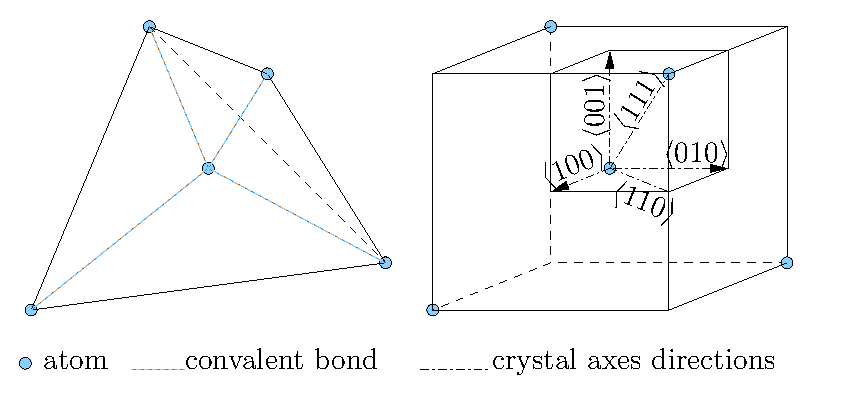
\includegraphics[width=0.6\textwidth]{xtalStruc}  
  \caption{Structure of germanium crystal.}
  \label{fig:xtal}
\end{figure}

Due to the crystal lattice symmetry in germanium, in three directions, the crystallographic $\langle100\rangle$, $\langle110\rangle$ and $\langle111\rangle$, the mobility is always aligned with the electrical field. Consequently, the drift velocity is aligned with the symmetry axis as well. Therefore we can obtain the longitudinal anisotropy of the drift mobility in these special directions. Experimental data on the longitudinal anisotropy in these specific directions can be found in literature. The mobility data can be well fitted in any principal crystallographic direction with the parameterization:
\begin{equation}
  \label{eq:para}
  v = \frac{\mu_{0}E}{[1+(\frac{E}{E_{0}})^{\beta}]^{1/\beta}} -   \mu_{n}E,
\end{equation}
where $E, v$ are the magnitudes of the electric field and drift velocity, respectively, $\mu_{0}, \mu_{n}, E_{0}$ and $\beta$ are the fitting parameters. At low fields, the mobility becomes isotropic and therefore the mobility fit parameter $\mu_{0}$ is expected to become independent of the crystallographic direction. For hot electrons, the departure from a linear $v \sim E$ relation is modeled through the parameters $E_{0}$ and $\beta$. At high field, Mihailescu \textit{et   al.}~\cite{miha} have added the term $\mu_{n}E$ to account for the \emph{Gunn effect} that was observed by Ottaviani \textit{et   al.}~\cite{otta} for field strengths above 3~kV$/$cm at 80~K. However, this effect is insignificant in our detector operated with field strengths 0.1-3~kV$/$cm. Parameterization values fitted with the experimental data are summarized in Table~\ref{tab:pars}. The values from two different references are quite different from each other. We'd better measure it by ourselves again.

\begin{table}[tbhp]
  \centering
  \begin{tabular}{ccccccc}\hline\hline
     Reference & Carrier & Direction & $\mu_{0} \left[ \frac{\mbox{cm}^{2}}{\mbox{V}\cdot\mbox{s}} \right]$ & $E_{0} \left[ \frac{\mbox{V}}{\mbox{cm}} \right]$ & $\beta$ & $\mu_{n} \left[ \frac{\mbox{cm}^{2}}{\mbox{V}\cdot\mbox{s}} \right]$ \\\hline
& Electron & $\langle111\rangle$ & 40180 & 493 & 0.72 & 589 \\
Ref.~\cite{miha}& & $\langle100\rangle$ & 42420 & 251 & 0.87 & 62\\
& Hole & $\langle111\rangle$ & 107270 & 100 & 0.58 & - \\
& & $\langle100\rangle$ & 66333 & 181 & 0.744 & - \\\hline\hline
& Electron & $\langle111\rangle$ & 38536 & 538 & 0.641 & 510 \\
Ref.~\cite{bart}& & $\langle100\rangle$ & 38609 & 511 & 0.805 & -171\\ 
& Hole & $\langle111\rangle$ & 61215 & 182 & 0.662 & - \\
& & $\langle100\rangle$ & 61824 & 185 & 0.942 & - \\\hline\hline
  \end{tabular}
  \caption{Fit parameters for the experimental drift velocities in the 
$\langle111\rangle$ and $\langle100\rangle$ directions.}
\label{tab:pars}
\end{table}

The anisotropy in any direction is related to the longitudinal anisotropy in the $\langle100\rangle$ and $\langle111\rangle$ directions. The drift velocity in any direction can be calculated accordingly. The detailed calculation will be described in the following two sections.

It is very important to distinguish two different coordinate systems in the calculation. One is the coordinate defined by the crystal axes $\langle100\rangle$, $\langle010\rangle$ and $\langle001\rangle$. They are perpendicular to each other hence can be used as the axes of a Cartesian coordinate. The other one, indicated as $xyz$ in Fig~\ref{fig:coo}, is used in Geant4 geometry modeling. When you construct your detector as a Geant4 tube, the locate coordinate system attached to this tube is shown in Fig~\ref{fig:coo} as $xyz$. Our germanium detector has a cylindrical shape. The crystal is produced such that its $\langle001\rangle$ axis is aligned with the middle axis of the cylinder, \textit{i.e.} aligned with the z-axis of the coordinate used in Geant4 simulation. So the relation between the two coordinates can be described by an angle between the $\langle110\rangle$ axis and the y-axis, $\phi_{110}$.
\begin{figure}[htpb]
  \centering
  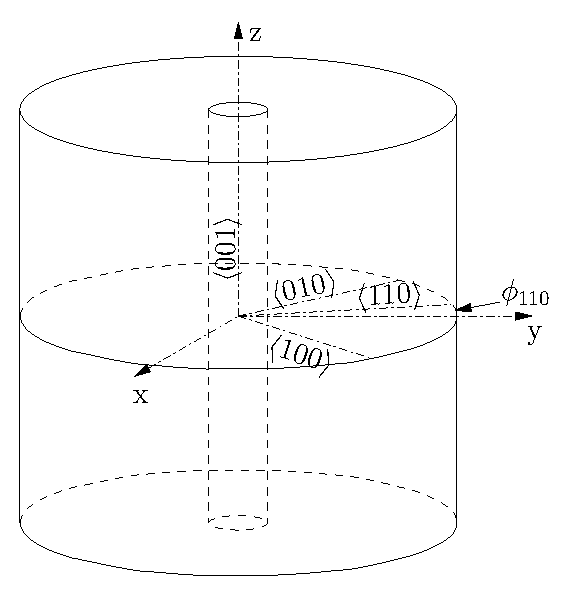
\includegraphics[width=0.3\textwidth]{coordins}  
  \caption{The relation between the coordinate $xyz$ used in Geant4     simulation and the one defined by the crystal axes     $\langle100\rangle$, $\langle010\rangle$ and $\langle001\rangle$.}
  \label{fig:coo}
\end{figure}

\subsubsection{Electron drift velocity}
\label{sec:elec}
There are four ellipsoidal valleys in the germanium crystal lying along the $\langle111\rangle$ directions as shown in Fig~\ref{fig:valley}. Electrons mostly populate in them and can be easily accelerated by the external electrical field. The population of electrons in other directions is very small and is neglected in the following calculation.
\begin{wrapfigure}{O}{0.4\textwidth}
  \centering
  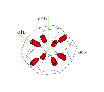
\includegraphics[width=0.4\textwidth]{valleys}  
  \caption{Four ellipsoidal valleys along $\langle111\rangle$     directions, where electrons mostly populate.}
  \label{fig:valley}
\end{wrapfigure}

Only considering the effect of the four ellipsoidal valleys shown in Fig~\ref{fig:valley}, the dependence of the electron drift velocity $\mathbf{v}_{e}$ on the applied electric field $\mathbf{E}$ is taken to be
\begin{equation}
  \label{eq:ed}
  \mathbf{v}_{e}(\mathbf{E}) = \mathcal{A}(E) \sum_{j}     \frac{n_{j}}{n} \frac{\gamma_{j}\mathbf{E_{0}}}           {\sqrt{\mathbf{E_{0}}\gamma_{j}\mathbf{E_{0}}}}, \mbox{ with }           j=1,2,3,4
\end{equation}
where $\mathcal{A}$ is a function of the magnitude of the electric field $E=|\mathbf{E}|$ and temperature, the value of $\mathcal{A}$ must be negative because electrons drift to the opposite direction of the electric field; $\mathbf{E_{0}}$ is the normalized electric field vector; $n_{j}/n$ is the fraction of the carriers (in this case, electrons) in the $j$-th $\langle111\rangle$ valley, $\gamma_{j}$ is the effective mass tensor for the $j$-th $\langle111\rangle$ valley. In the local coordinate of one of the ellipsoidal valleys $x^{\prime}y^{\prime}z^{\prime}$, as shown in Fig.~\ref{fig:axes}, the effective mass tensor has a very simple expression:
\begin{equation}
  \label{eq:gamma0}
  \gamma_{0} \equiv \left(
    \begin{array}{ccc}
      m_{t}^{-1} & 0 & 0 \\
      0 & m_{l}^{-1} & 0 \\
      0 & 0 & m_{t}^{-1}
    \end{array} \right),
\end{equation}
where $m_{t} = 1.64m_{e}$ is the transversal effective electron mass, $m_{l} = 0.0819m_{e}$ is the longitudinal effective electron mass, with $m_{e}$ denoting the free electron mass. Since it is convenient to simulate the interactions and the pulse shape developing in the same coordinate $xyz$, as shown in Fig.~\ref{fig:coo} and \ref{fig:axes}, we have to calculate the expressions of $\gamma_{j}$'s in $xyz$:
\begin{equation}
  \label{eq:gammas}
  \gamma_{j} = R_{j}^{-1}\gamma_{0}R_{j} = R_{j}^{T}\gamma_{0}R_{j},
\end{equation}
where
\begin{equation}
  \label{eq:rs}
  R_{j} = R_{x^{\prime}}(\arccos(\sqrt{2/3}))R_{z}(\phi_{110}+(j-1)\pi/2)
\end{equation}
is the rotation matrix which could align $\langle111\rangle$ axis to the y-axis. The suffix of $R$'s indicate the rotation axes. The rotation angles are denoted in the brackets following the $R$'s. All the rotations are defined in the counter-clockwise sense.

\begin{figure}[tbhp]
  \centering
  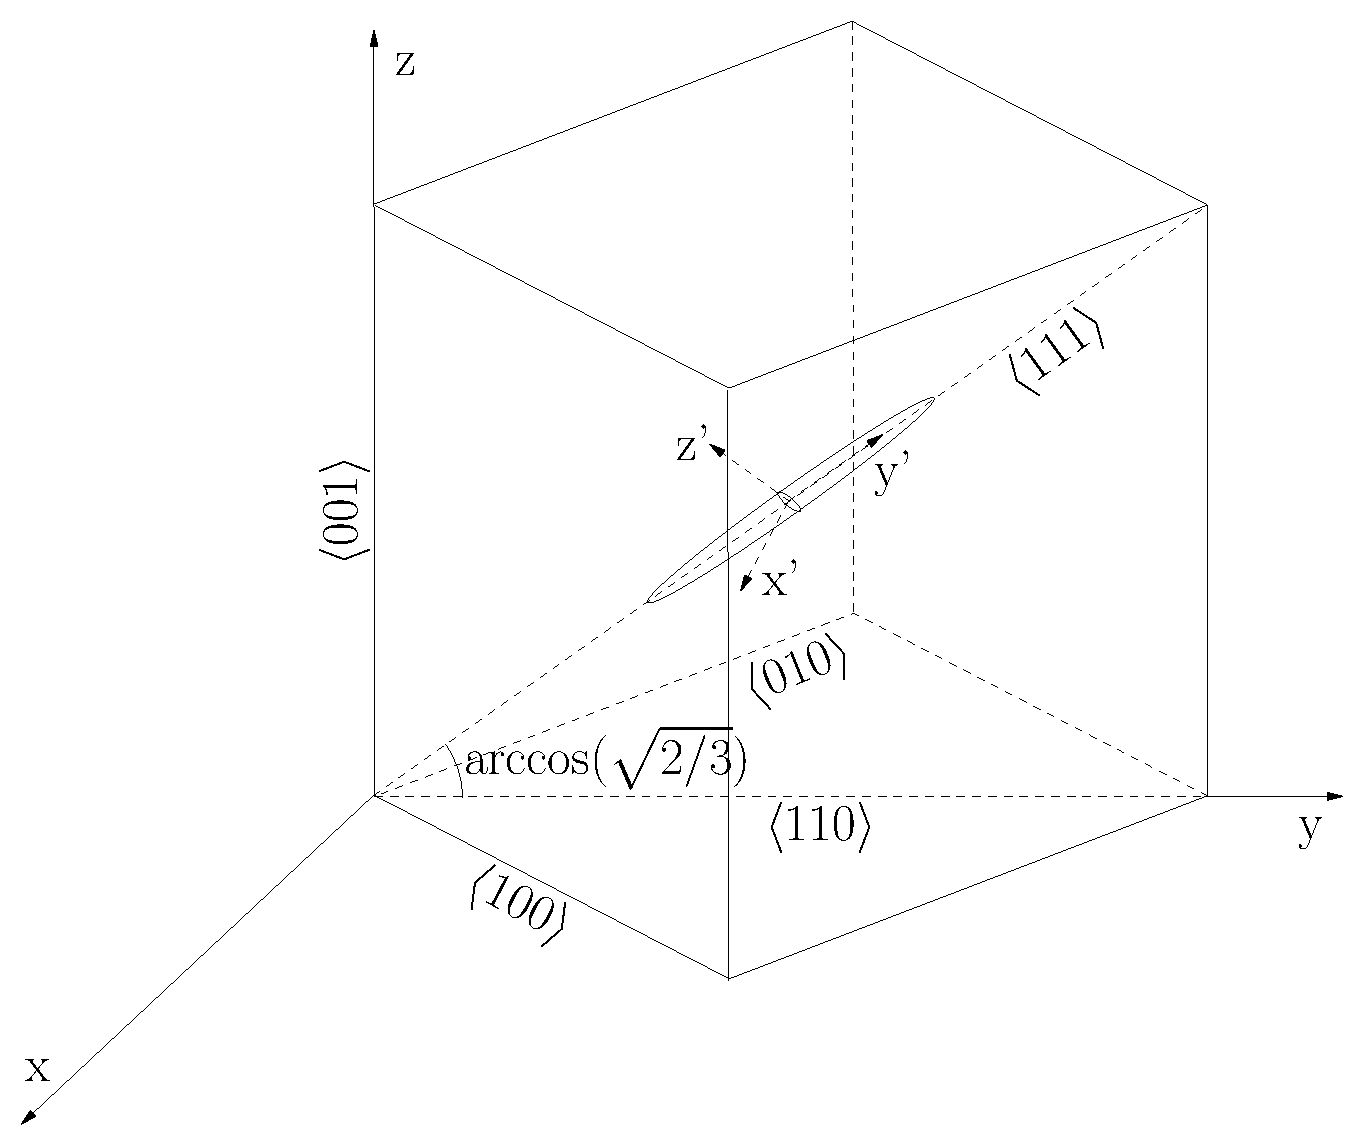
\includegraphics[width=0.4\textwidth]{axes}  
  \caption{Relation between the local coordinate     $x^{\prime}y^{\prime}z^{\prime}$ of one of the four ellipsoidal     valleys and the Geant4 coordinate $xyz$. The $x^{\prime}$ axis is     perpendicular to the plane defined by $\langle111\rangle$ and     $\langle001\rangle$.}
  \label{fig:axes}
\end{figure}

For an experimental determination of the repopulation amplitude, the deviation from a uniform population distribution $n_{e}/n$ (1/4 for germanium) is assumed to vary with the electric field weighted by the factor $\mathcal{R}$:
\begin{equation}
  \label{eq:nion}
  \frac{n_{j}}{n} = \mathcal{R}(E)   \left[         \frac{\sqrt{\mathbf{E_{0}}\gamma_{j}\mathbf{E_{0}}}}
    {\sum_{i}\sqrt{\mathbf{E_{0}}\gamma_{i}\mathbf{E_{0}}}} -               \frac{n_{e}}{n} \right] + \frac{n_{e}}{n}, 
\end{equation}

If the electric field vector is equally oriented with respect to all the $\langle111\rangle$ directions, there is an uniform repopulation of the conduction bands, \textit{i.e.} $n_{j}/n = 1/4$. An electric field applied along the $\langle100\rangle$ direction, \textit{i.e.} $\mathbf{E_{0}} = (\sqrt{1/2},\sqrt{1/2},0)^{T}$ in coordinate $xyz$, satisfies this condition. By employing the experimental drift velocity $v_{e}^{100}(E)$ which can be calculated using Eq.~\ref{eq:para}, the absolute value of $\mathcal{A}(E)$ can be calculated as
\begin{equation}
  \label{eq:ae}
  |\mathcal{A}(E)| = \frac{v_{e}^{100}(E)}  {\displaystyle \sum_{j}     \frac{1}{4}     \frac{\gamma_{j}\mathbf{E_{0}}}         {\sqrt{\mathbf{E_{0}}\gamma_{j}\mathbf{E_{0}}}} },  \mbox{ with }       \mathbf{E_{0}} = \left( \begin{array}{c} 
    \sqrt{1/2}\\\sqrt{1/2}\\0 \end{array} \right).
\end{equation}

If the electric field vector is oriented along with one of the $\langle111\rangle$ directions, \textit{i.e.} $\mathbf{E_{0}} = (0,\sqrt{2/3},\sqrt{1/3})^{T}$ in coordinate $xyz$, there is an uniform repopulation of the conduction bands among the other three $\langle111\rangle$ axes, \textit{i.e.}
\begin{equation}
  \label{eq:n111}
  \frac{n_{2}}{n} = \frac{n_{3}}{n} = \frac{n_{4}}{n}.
\end{equation}
Since
\begin{equation}
  \label{eq:nsum}
  \displaystyle \sum_{j}\frac{n_{j}}{n} = 1,
\end{equation}
we have
\begin{equation}
  \label{eq:n12}
  \frac{n_{1}}{n} + 3\frac{n_{2}}{n}= 1.
\end{equation}
By employing the experimental drift velocity $v_{e}^{111}(E)$ for an applied electric field $E$ in the $\langle111\rangle$ direction at a specific temperature, which can be calculated using Eq.~\ref{eq:para}, we have another relation between $n_{1}/n$ and $n_{2}/n$:
\begin{equation}
  \label{eq:n12p}
  v_{e}^{111}(E) =  \mathcal{A}(E) \left(  \frac{n_{1}}{n} \frac{\gamma_{1}\mathbf{E_{0}}}         {\sqrt{\mathbf{E_{0}}\gamma_{1}\mathbf{E_{0}}}} +  3\frac{n_{2}}{n} \frac{\gamma_{2}\mathbf{E_{0}}}         {\sqrt{\mathbf{E_{0}}\gamma_{2}\mathbf{E_{0}}}} \right).
\end{equation}
One can get the value of $n_{1}/n$ and $n_{2}/n$ by solving the equations \ref{eq:n12} and \ref{eq:n12p} together. Then $\mathcal{R}(E)$ can be calculated as
\begin{equation}
  \label{eq:re}
  \mathcal{R}(E) = \left( \frac{n_{1}}{n} - \frac{n_{e}}{n} \right) / \left( \frac{\sqrt{\mathbf{E_{0}}\gamma_{1}\mathbf{E_{0}}}}
    {\sum_{j}\sqrt{\mathbf{E_{0}}\gamma_{j}\mathbf{E_{0}}}} -                           \frac{n_{e}}{n} \right), \mbox{ with } \mathbf{E_{0}} = \left( \begin{array}{c} 
  0\\ \sqrt{2/3}\\\sqrt{1/3} \end{array} \right).
\end{equation}

After determination of the parameters $\mathcal{A}$ and $\mathcal{R}$, the drift velocity can be calculated for any direction and any strength of the electric field.

\subsubsection{Hole drift velocity}
\label{sec:hole}
The model used in calculating the hole drift velocity is taken from Ref.~\cite{bart}. In this model the so-called heavy hole valence band is solely responsible for the anisotropic mobility while the other effects are neglected. The holes are accelerated in the electrical field until their energy becomes 0.037~eV. At this point their energy is sufficiently large to emit an optical phonon, a process which is very likely to happen. By emitting an optical phonon, the hole typically loses most of its energy and resumes acceleration in the field direction and a new cycle starts. 

From this picture, the properties of the probability distribution function for finding a heavy hole in a specific momentum state, $\mathbf{k}$, can be predicted. The distribution should peak in the direction in which $\mathbf{k}$ is parallel to the electrical field. So the mean wave vector $\mathbf{k}_{0}(k_{0}, \theta_{0}, \phi_{0})$ is assumed to be aligned with the applied electrical field $\mathbf{E}(E, \theta, \phi)$, \textit{i.e.} $\theta_{0} = \theta, \phi_{0} = \phi$, where $\theta, \phi$ are the polar and azimuthal angles with respect to the coordinate defined by the $\langle100\rangle$, $\langle010\rangle$ and $\langle001\rangle$ axes as shown in Fig.~\ref{fig:vsphere}.
\begin{figure}[tbhp]
  \centering
  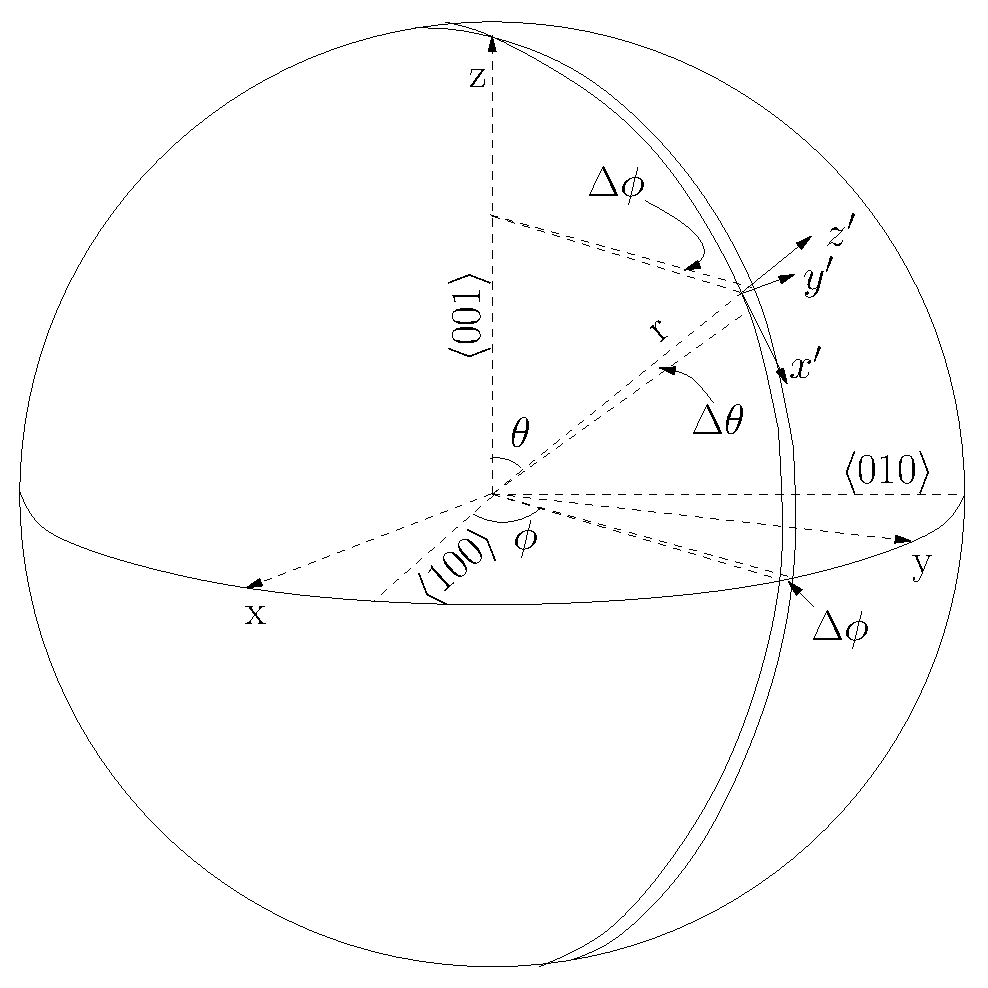
\includegraphics[width=0.4\textwidth]{vsphere}  
  \caption{Relation between the coordinate defined by the crystal
$\langle100\rangle$, $\langle010\rangle$ and $\langle001\rangle$ axes,
the one used in the Geant4 simulation, $xyz$ and the local coordinate
$x^{\prime}y^{\prime}z^{\prime}$ attached to each position.}
  \label{fig:vsphere}
\end{figure}

The three components $(v_{x^{\prime}}, v_{y^{\prime}}, v_{z^{\prime}})^{T}$ of the hole drift velocity $\mathbf{v}$ in the local coordinate $x^{\prime}y^{\prime}z^{\prime}$ at any position $(r, \theta, \phi)$ (as shown in Fig.~\ref{fig:vsphere}) can be expressed as:
\begin{equation}
  \label{eq:vsphere}
  \begin{array}{rcl}
   v_{x^{\prime}} = v_{r} &=& v^{100}_{h}(E)[1-\Lambda(k_{0})(\sin(\theta)^{4}\sin(2\phi)^{2} + \sin(2\theta)^{2})],\\
   v_{y^{\prime}} = v_{\theta} &=& v^{100}_{h}(E)\Omega(k_{0})[2\sin(\theta)^{3}\cos(\theta)\sin(2\phi)^{2} + \sin(4\theta)],\\
    v_{z^{\prime}} = v_{\phi} &=& v^{100}_{h}(E)\Omega(k_{0})\sin(\theta)^{3}\sin(4\phi).
  \end{array}
\end{equation}
The mean wave number $k_{0}$ can be expressed as a function of $v_{rel} = v^{111}_{h}(E)/v^{100}_{h}(E)$:
\begin{equation}
  \label{eq:k0}
   k_{0}(v_{rel}) = 9.2652 - 26.3467v_{rel} + 29.6137v_{rel}^{2} - 12.3689v_{rel}^{3},
\end{equation}
where $v^{111}_{h}(E)$ and $v^{100}_{h}(E)$ indicate the drift velocity along the $\langle111\rangle$ and $\langle100\rangle$ direction. They can be calculated using Eq.~\ref{eq:para}. The function $\Lambda$ and $\Omega$ govern the amplitude of the anisotropy and can be expressed as
\begin{equation}
  \label{eq:lamb}
   \Lambda(k_{0}) = -0.01322k_{0} + 0.41145k_{0}^{2} - 0.23657k_{0}^{3} + 0.04077k_{0}^{4},
\end{equation}
\begin{equation}
  \label{eq:ome}
   \Omega(k_{0}) = 0.006550k_{0} - 0.19946k_{0}^{2} + 0.09859k_{0}^{3} - 0.01559k_{0}^{4}.
\end{equation}

The three components $(v_{x}, v_{y}, v_{z})^{T}$ of the hole drift velocity $\mathbf{v}$ in the coordinate $xyz$ (as shown in Fig.~\ref{fig:vsphere}) can be calculated as:
\begin{equation}
  \label{eq:v2v}  
  \left(
    \begin{array}{c}
      v_{x} \\ v_{y} \\ v_{z}
    \end{array}
\right) = R_{z}(\phi + \frac{\pi}{4} + \phi_{110}) R_{y^{\prime}}(\theta) \left( 
    \begin{array}{c}
      v_{x^{\prime}} \\ v_{y^{\prime}} \\ v_{z^{\prime}}
    \end{array} \right),
\end{equation}
where $R$'s indicate the rotation matrix along a specific axis, such as $y^{\prime}$ or $z$. The rotation angles are denoted in the following brackets. All the rotations are defined in the counter-clockwise sense.

%%% Local Variables:
%%% mode:latex
%%% TeX-master: "GSTR-08-M007"
%%% End:
